\documentclass{beamer}
\usetheme{Madrid}
\usecolortheme{default}

% Additional packages
\usepackage{graphicx}
\usepackage{amsmath}
\usepackage{listings}
\usepackage{xcolor}
\usepackage{subcaption}

% Custom colors and styles
\definecolor{codegreen}{rgb}{0,0.6,0}
\definecolor{codegray}{rgb}{0.5,0.5,0.5}
\definecolor{backcolour}{rgb}{0.95,0.95,0.92}

\lstdefinestyle{mystyle}{
    backgroundcolor=\color{backcolour},   
    commentstyle=\color{codegreen},
    basicstyle=\ttfamily\small,
    breakatwhitespace=false,         
    breaklines=true,                 
    keepspaces=true,                 
    showspaces=false,                
    showstringspaces=false,
    showtabs=false,                  
    tabsize=2
}
\lstset{style=mystyle}

\title{Neural Implicit Flow: A Comparative Study}
\subtitle{Implementation Approaches and Performance Analysis}
\author{Christian Beneke}
\date{10.02.2025}

\begin{document}

\begin{frame}
    \titlepage
\end{frame}

\begin{frame}{Outline}
    \tableofcontents
\end{frame}

\section{Introduction}
\begin{frame}{Problem Space \& Motivation}
    \begin{itemize}
        \item High-dimensional spatio-temporal dynamics are computationally challenging
        \item Traditional methods face limitations:
        \begin{itemize}
            \item Fixed mesh structures (SVD, CAE)
            \item Poor scaling with high-dimensional data
            \item Limited ability to capture nonlinear dynamics
        \end{itemize}
        \item Real-world applications require:
        \begin{itemize}
            \item Adaptive mesh handling
            \item Efficient dimensionality reduction
            \item Real-time processing capabilities
        \end{itemize}
    \end{itemize}
\end{frame}

\begin{frame}{Key Challenges in Current Approaches}
    \begin{itemize}
        \item Singular Value Decomposition (SVD)
        \begin{itemize}
            \item Limited to fixed mesh structures
            \item Poor scaling with dimensionality
        \end{itemize}
        \item Convolutional Autoencoders (CAE)
        \begin{itemize}
            \item Requires uniform grid resolution
            \item Struggles with adaptive meshing
        \end{itemize}
        \item Common Issues
        \begin{itemize}
            \item High computational overhead
            \item Limited expressiveness for complex dynamics
            \item Poor generalization to new scenarios
        \end{itemize}
    \end{itemize}
\end{frame}

\section{Neural Implicit Flow Framework}
\begin{frame}{Core Architecture}
    \begin{columns}
        \column{0.6\textwidth}
        \begin{itemize}
            \item Two specialized networks:
            \begin{itemize}
                \item ShapeNet: Spatial complexity
                \item ParameterNet: Temporal evolution
            \end{itemize}
            \item Key innovations:
            \begin{itemize}
                \item Mesh-agnostic representation
                \item Efficient parameter sharing
                \item Adaptive complexity handling
            \end{itemize}
        \end{itemize}
        
        \column{0.4\textwidth}
        \begin{figure}
            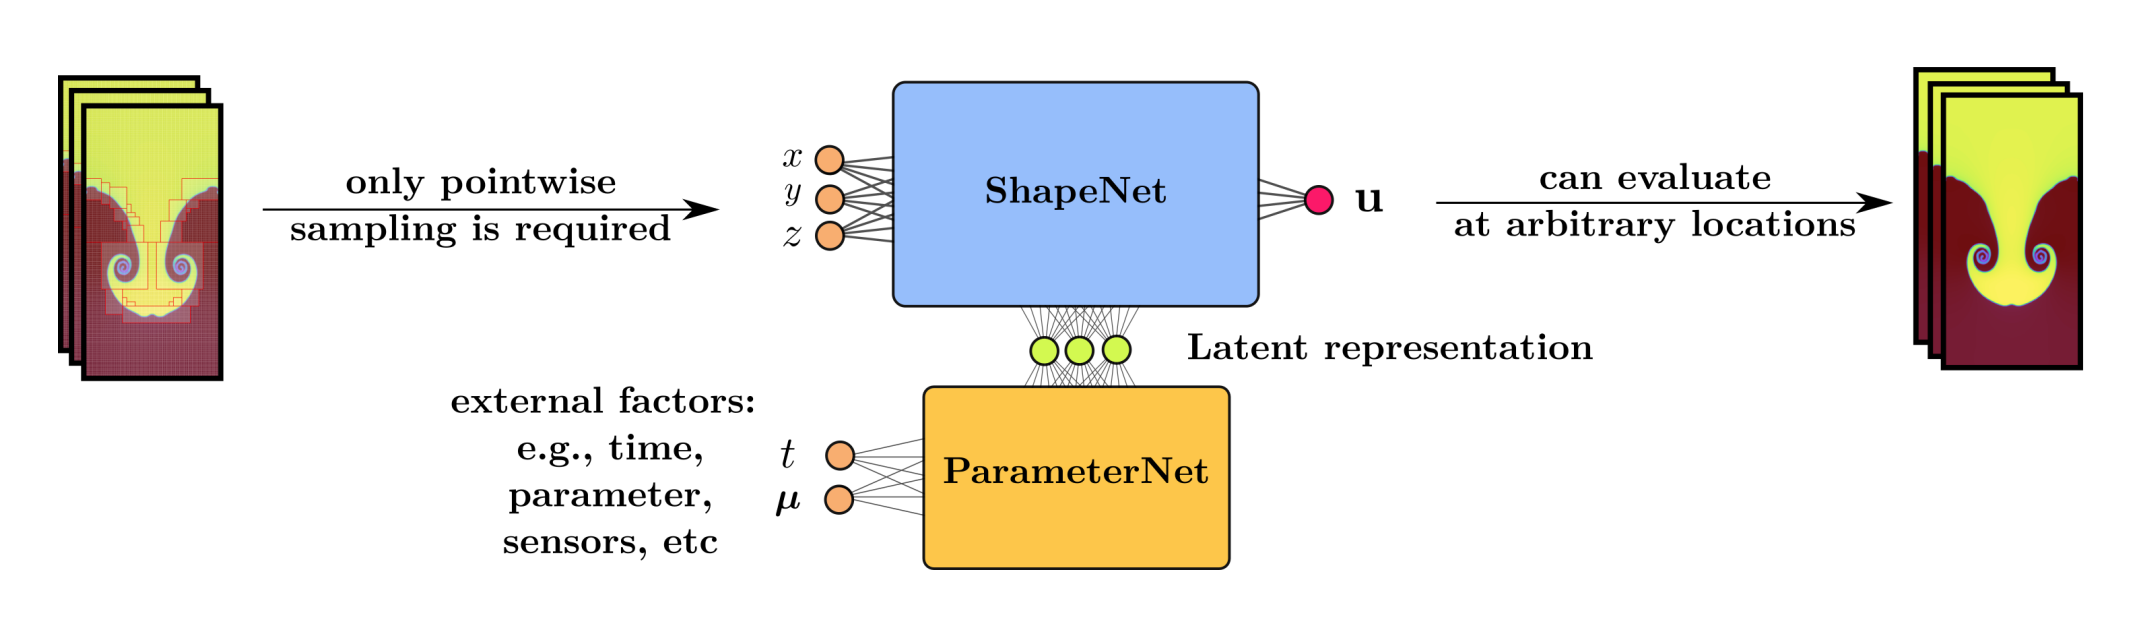
\includegraphics[width=\textwidth]{hypernetwork_diagram.png}
            \caption{NIF Architecture}
        \end{figure}
    \end{columns}
\end{frame}

\begin{frame}{Mathematical Formulation}
    \begin{itemize}
        \item Core mapping function:
        \[ f_\theta: (\mathbf{x}, \mathbf{t}) \mapsto u(\mathbf{x}, \mathbf{t}) \]
        where:
        \begin{itemize}
            \item $\mathbf{x} \in \mathbb{R}^d$: Spatial coordinate
            \item $\mathbf{t} \in \mathbb{R}^p$: Temporal/parametric input
            \item $u$: Field value
        \end{itemize}
        \item Hypernetwork decomposition:
        \[ f_\theta(\mathbf{x}, \mathbf{t}) = \text{ShapeNet}_{\text{ParameterNet}_{\theta_p}(\mathbf{t})}(\mathbf{x}) \]
    \end{itemize}
\end{frame}

\section{Implementation Approaches}
\begin{frame}{Implementation Overview}
    \begin{itemize}
        \item Three distinct implementations:
        \begin{itemize}
            \item Upstream Reference (TensorFlow)
            \item TensorFlow Functional API
            \item PyTorch Implementation
        \end{itemize}
        \item Key considerations:
        \begin{itemize}
            \item Framework-specific optimizations
            \item Code maintainability
            \item Development ergonomics
        \end{itemize}
    \end{itemize}
\end{frame}

\begin{frame}{Upstream Reference Implementation}
    \begin{itemize}
        \item Based on original paper implementation
        \item Key modifications:
        \begin{itemize}
            \item Migration to modern TensorFlow patterns
            \item Improved gradient tape management
            \item Enhanced base class structure
        \end{itemize}
        \item Code example:
        \begin{lstlisting}[language=Python]
class HyperLayer(tf.keras.layers.Layer):
    def __init__(self, weights_from, weights_to,
                 bias_offset, biases_from, biases_to):
        self.weights_from = weights_from
        self.weights_to = weights_to
        self.biases_from = bias_offset + biases_from
        self.biases_to = bias_offset + biases_to
        \end{lstlisting}
    \end{itemize}
\end{frame}

\begin{frame}{TensorFlow Functional API Implementation}
    \begin{itemize}
        \item Complete architectural redesign
        \item Key features:
        \begin{itemize}
            \item Functional programming principles
            \item Improved composability
            \item XLA compilation support
        \end{itemize}
        \item Optimizations:
        \begin{itemize}
            \item Vectorized weight generation
            \item Memory-efficient parameter handling
            \item Mixed precision training (FP16/FP32)
        \end{itemize}
    \end{itemize}
\end{frame}

\begin{frame}{PyTorch Implementation}
    \begin{itemize}
        \item Modern PyTorch features:
        \begin{itemize}
            \item Dynamic computation graphs
            \item Native autograd functionality
            \item Improved debugging capabilities
        \end{itemize}
        \item Implementation highlights:
        \begin{itemize}
            \item Flexible activation mapping
            \item Efficient static weight layers
            \item Comprehensive training logger
        \end{itemize}
    \end{itemize}
\end{frame}

\section{Experimental Setup}
\begin{frame}{Test Cases}
    \begin{columns}
        \column{0.6\textwidth}
        \textbf{Low Frequency Wave}
        \begin{itemize}
            \item Domain: $x \in [0,1]$, $t \in [0,100]$
            \item 200 spatial points, 10 timesteps
            \item Simple periodic traveling wave
            \item $u(x,t) = \exp(-1000(x-x_0-ct)^2)$
        \end{itemize}
        
        \column{0.4\textwidth}
        \begin{figure}
            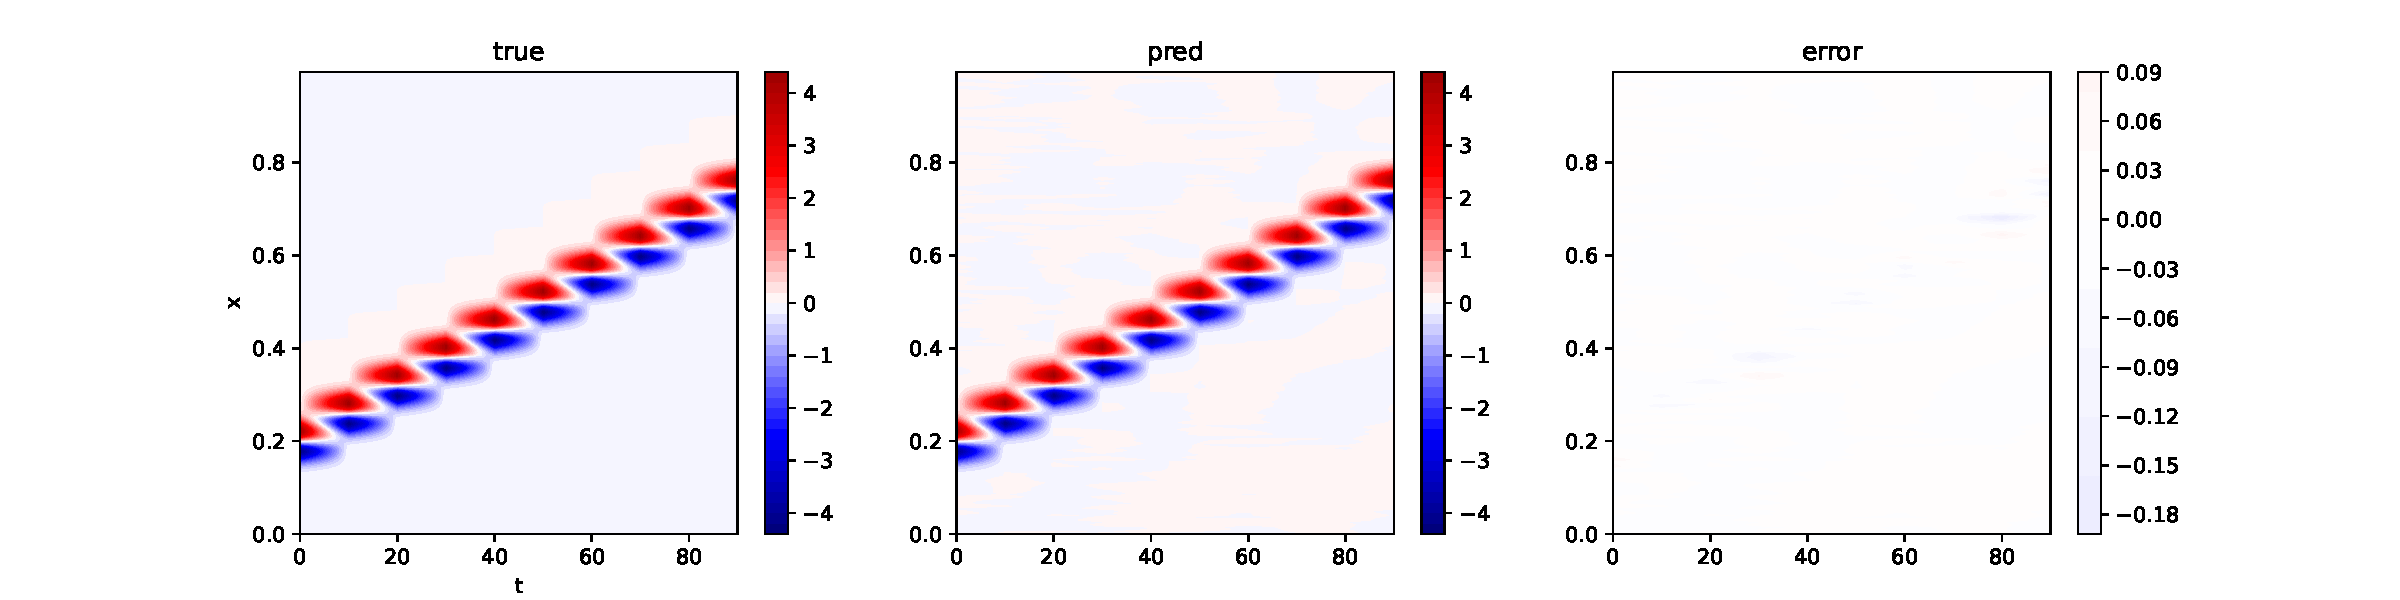
\includegraphics[width=\textwidth]{../../results/functional/low-frequency-adam-20250206-1105-1/vis}
            \caption{Low Frequency Example}
        \end{figure}
    \end{columns}
\end{frame}

\begin{frame}{Test Cases (cont.)}
    \begin{columns}
        \column{0.6\textwidth}
        \textbf{High Frequency Wave}
        \begin{itemize}
            \item Same spatial/temporal domain
            \item Added frequency $\omega = 400$
            \item Complex oscillatory pattern
            \item $u(x,t) = \exp(-1000(x-x_0-ct)^2)\sin(\omega(x-x_0-ct))$
        \end{itemize}
        
        \column{0.4\textwidth}
        \begin{figure}
            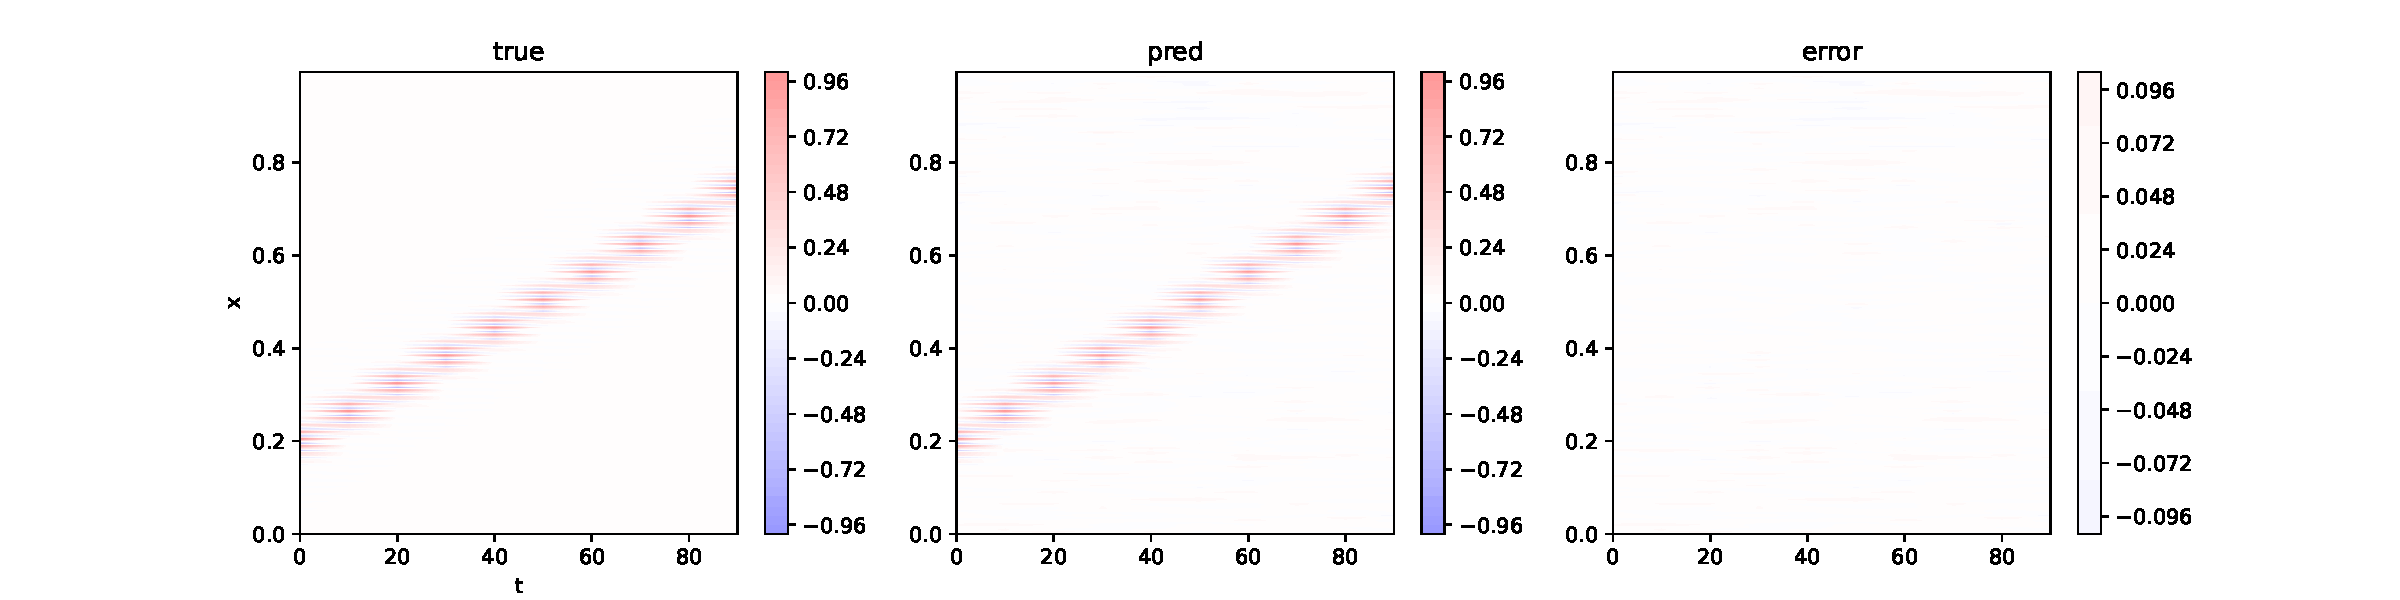
\includegraphics[width=\textwidth]{../../results/functional/high-frequency-adam-20250206-1520-1/vis}
            \caption{High Frequency Example}
        \end{figure}
    \end{columns}
\end{frame}

\begin{frame}{Network Architectures}
    \begin{columns}
        \column{0.5\textwidth}
        \textbf{ParameterNet}
        \begin{itemize}
            \item Dense input layer
            \item Two hidden layers (30 units)
            \item Single-unit bottleneck
            \item Adaptive output layer
        \end{itemize}
        
        \column{0.5\textwidth}
        \textbf{ShapeNet Variants}
        \begin{itemize}
            \item Shortcut (Low frequency)
            \begin{itemize}
                \item Skip connections
                \item Swish activation
            \end{itemize}
            \item SIREN (High frequency)
            \begin{itemize}
                \item Sinusoidal activation
                \item $\omega_0 = 30$ scaling
            \end{itemize}
        \end{itemize}
    \end{columns}
\end{frame}

\section{Results and Analysis}
\begin{frame}{Performance Overview}
    \begin{itemize}
        \item Low Frequency Results:
        \begin{itemize}
            \item TF Functional API (Adam): 1.526e-04
            \item PyTorch (Adam): 1.549e-04
            \item Upstream (AdaBelief): 5.073e-04
        \end{itemize}
        \item High Frequency Results:
        \begin{itemize}
            \item PyTorch (Adam): 1.884e-04
            \item TF Functional API (Adam): 5.415e-04
            \item Upstream: Not available
        \end{itemize}
    \end{itemize}
\end{frame}

\begin{frame}{Processing Speed Comparison}
    \begin{table}
        \centering
        \begin{tabular}{lcc}
            \hline
            \textbf{Implementation} & \textbf{Low Freq.} & \textbf{High Freq.} \\
            \hline
            TF Functional & 11.5-17K pts/s & 11.5-16K pts/s \\
            PyTorch & 12-15K pts/s & 6-16K pts/s \\
            Upstream & 12-17K pts/s & - \\
            \hline
        \end{tabular}
        \caption{Processing Speed (points per second)}
    \end{table}
\end{frame}

\begin{frame}{Optimizer Impact}
    \begin{itemize}
        \item Adam vs AdaBelief comparison:
        \begin{itemize}
            \item TF Functional API: 62.5\% improvement
            \item PyTorch: 5.10x improvement (low freq.)
            \item PyTorch: 11.77x improvement (high freq.)
        \end{itemize}
        \item Key findings:
        \begin{itemize}
            \item Adam: More stable convergence
            \item Better final loss values
            \item Consistent across implementations
        \end{itemize}
    \end{itemize}
\end{frame}

\begin{frame}{Visual Results - Low Frequency}
    \begin{figure}
        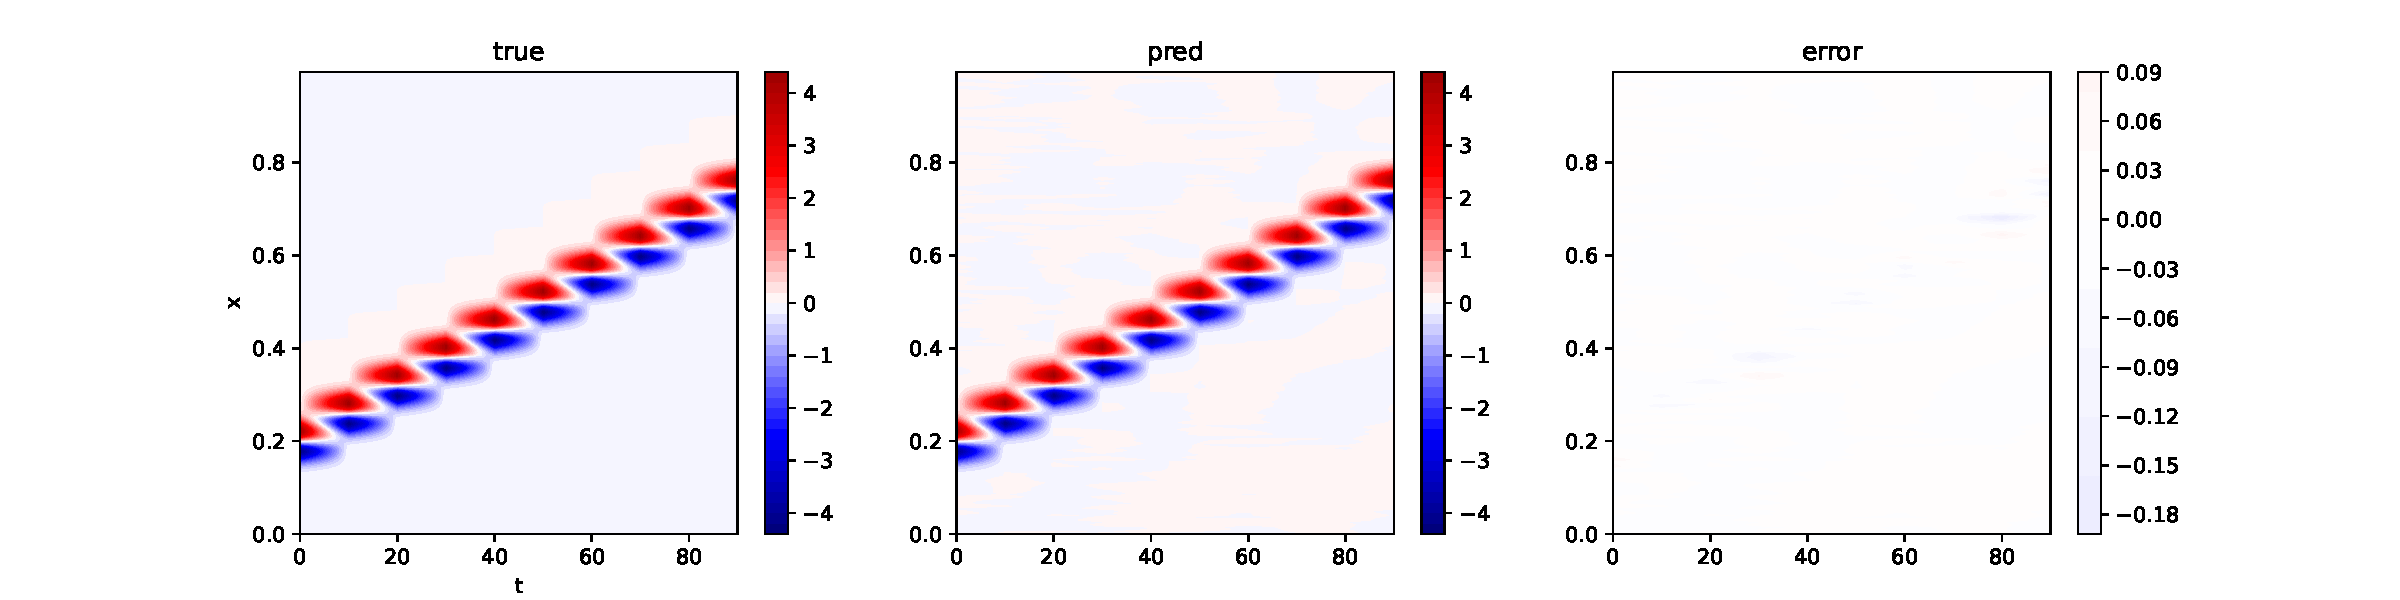
\includegraphics[width=\textwidth]{../../results/functional/low-frequency-adam-20250206-1105-1/vis}
        \caption{Low Frequency Predictions (TF Functional API)}
    \end{figure}
\end{frame}

\begin{frame}{Visual Results - High Frequency}
    \begin{figure}
        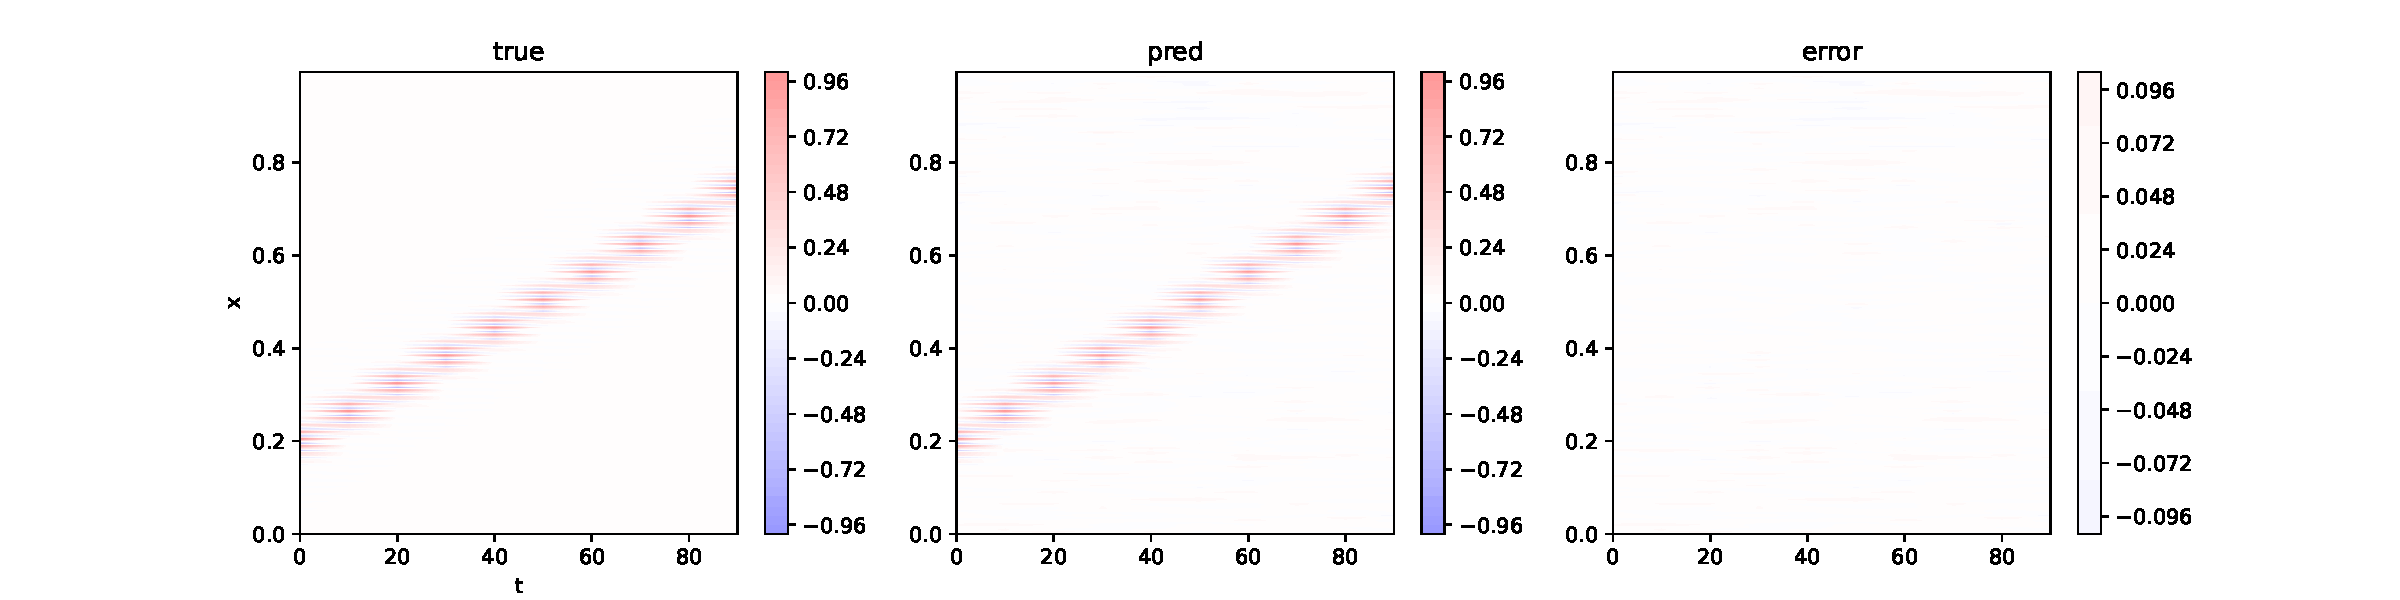
\includegraphics[width=\textwidth]{../../results/functional/high-frequency-adam-20250206-1520-1/vis}
        \caption{High Frequency Predictions (TF Functional API)}
    \end{figure}
\end{frame}

\section{Conclusions}
\begin{frame}{Key Findings}
    \begin{itemize}
        \item Implementation Trade-offs:
        \begin{itemize}
            \item Modern implementations excel at high-frequency cases
            \item TF Functional API: Most consistent performance
            \item PyTorch: Best high-frequency accuracy
        \end{itemize}
        \item Practical Implications:
        \begin{itemize}
            \item All implementations achieve production-ready speed
            \item Adam optimizer consistently outperforms AdaBelief
            \item Framework choice impacts development experience
        \end{itemize}
    \end{itemize}
\end{frame}

\begin{frame}{Future Directions}
    \begin{itemize}
        \item Technical Improvements:
        \begin{itemize}
            \item Additional network architectures
            \item Memory optimization
            \item Computational efficiency
        \end{itemize}
        \item Application Areas:
        \begin{itemize}
            \item Fluid dynamics
            \item Climate modeling
            \item Materials science
        \end{itemize}
        \item Research Opportunities:
        \begin{itemize}
            \item Complex spatio-temporal problems
            \item Multi-scale phenomena
            \item Real-time applications
        \end{itemize}
    \end{itemize}
\end{frame}

\begin{frame}
    \centering
    \Huge Thank you for your attention!
    
    \vspace{1cm}
    \Large Questions?
\end{frame}

\end{document}
